\chapter{LL and LR algorithms}
\label{chap:ll_and_lr}
This chapter is interested in how to parse CFGs grammar. We will see two
algorithms : LL and LR. Note that, they are not generic algorithms for CFGs
parsing.

\section{Historical perspective}
    \begin{itemize}
        \item Chomsky's Hierarchy : mid-50s
        \item LL \& LR : formalized in mid/late 60
        \item Processors at this time where not very efficient
        \item $\mathcal{O}(n^3)$ was laughable, way to slow
    \end{itemize}

    Taking that into account, the choice to make efficient implementation (no
    backtracking / fancy data structure) that can only parse a part of CFGs was
    made. It is very practical, indeed we can show that programming language
    typically can be parse in $\mathcal{O}(n)$.
\section{LL}
    \theoremstyle{definition}
    \begin{definition}[LL]
        LL = Left-to-right Leftmost derivation. It always expand the left
        non-terminal first.
    \end{definition}
    It can parse a subset of CFGs :
        \begin{itemize}
            \item Choices: use k tokens of lookahead to decide (never backtrack)
            \item Nowadays we consider it as a worse PEG
            \item If the grammar is accepted by LL, it guarantees
            $\mathcal{O}(n)$, can be implemented based on table-based lookup
        \end{itemize}
    \subsection{Properties}
        \begin{itemize}
            \item Top down recursive descent algorithm as PEG (but only one
            choice alternative taken, depends on lookahead lookup)
            \item No left recursion allowed
            \item Like PEG : unambiguous
            \item No language hiding (\[A ::= a* a\] is not a valid language in LL)
            \item Less expressive than CFG or PEG (even than LR)
        \end{itemize}

        \theoremstyle{definition}
        \begin{definition}[LL Grammar]
            Grammar for which we can generate an LL parser (no FIRST/FIRST or
            FIRST/FOLLOW conflicts)
        \end{definition}
        \theoremstyle{definition}
        \begin{definition}[LL Language]
            A language that has a LL grammar (may have multiple grammars
            including non-LL ones.)
        \end{definition}
        \subsubsection{LL Conflicts}
            \paragraph{FIRST/FIRST conflit}
                \begin{itemize}
                    \item Choices starting with the same k tokens
                    \item $A ::= ab | ac (k=1)$
                \end{itemize}
            \paragraph{FIRST/FOLLOW conflit}
                \begin{itemize}
                    \item Choice can start or (if it is nullable) be followed by
                    the same k tokens ($S ::= X Y ; X ::= \epsilon | a; Y ::= a | b$)
                \end{itemize}

                We can avoid FIRST/FIRST with left-factoring (factor out the
                common part at the start of two choice alternatives)
                \begin{figure}[H]
                     \centering
                     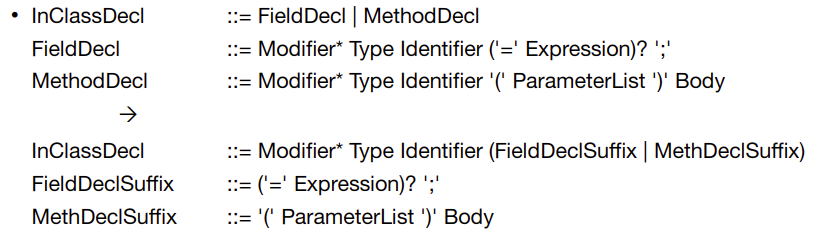
\includegraphics[scale=0.4]{LL_Conflict_avoid.png}
                     \caption{Left-factoring example}
                     \label{fig:left-factoring}
                \end{figure}
                
                In the previous figure, the three first line are not LL as the
                two last starts with the same prefix. The 3 last lines are LL
                because the suffix has been extracted, so the both use the same
                rule with a suffix choice instead of two rules.

                Note that it is not great for plain syntax tree, also makes the
                AST a bit more difficult to build. However it is also useful for
                PEG performance (we avoid parsing the same prefix many times).
    \subsection{LL(1) vs Regular Expression}
        As both of them use a single symbol we could ask why are they not the same.
        \begin{itemize}
            \item LL can handle central recursion
            \item Regular grammars are parser with $\mathcal{O}(1)$ space (current state)
            \item LL(1) implemented by top-down recursive descent uses
            $\mathcal{O}(n)$ space: the function call stack (can be use to
            recurse) 
        \end{itemize}
\section{LR}
    LR algorithm is the most difficult parsing algorithm that we'll see. Still,
    it is not the most difficult one (hello GLR). The goal of LR is to parse
    every deterministic grammar. Every grammar can be parsed in $\mathcal{O}(n)$
    without backtracking (we cannot explore different alternatives). Hence, it
    is not the same as LL(1) as LL(1) decides eagerly and ignores the context.

    \theoremstyle{definition}
    \begin{definition}[LR parsing]
        LR = Left-to-right Rightmost derivation.
        It always expand the right non-terminal first.

        Essentially done by DPDA:
            \begin{itemize}
                \item Stack on which symbols can be pushed (terminal and
                non-terminals)
                \item Performs a table lookup based on the stack and some tokens
                of lookahead(LL(1)/LL(k))
            \end{itemize}
    \end{definition}
    \subsection{Shift and reduce}
        The algorithm use a table that maps the stack to one of the two actions : 
        \begin{enumerate}
            \item shift : the next terminal onto the stack
            \item reduce : items at the top of the stack to a non-terminal.
        \end{enumerate}
        
        If we take our JSON grammar, an example would be :
        \begin{enumerate}
            \item remaining input \{ "x": 1\} Stack : []
            \item Shift x4 times
            \item Reduce to PAIR Stack : [ \{, "x", :, 1 ]
            \item Reduce to TPAIRS(from $\epsilon$) Stack : [ \{, PAIR ]
            \item Reduce to PAIRS Stack : [ \{, PAIR, TPAIRS ]
            \item Reduce to PAIRS? Stack : [ \{, PAIRS ]
            \item Shift Stack : [ \{, PAIRS? \}]
            \item Reduce to OBJECT Stack : [OBJECT] -> VALUE 
        \end{enumerate}
    \subsection{LR Conflicts}
        \paragraph{REDUCE/REDUCE conflicts}
            \begin{itemize}
                \item Rare case, it means the same set of symbols can be reduced
                to the same non-terminal, in the same context (same input prefix)
                \item Same portion of input could be matched to different non
                terminals (ambiguity)
                \item Non-trivial example can also appear using optional rules.
            \end{itemize}
        \paragraph{SHIFT/REDUCE conflicts}
            A famous problem for this is 
            \begin{lstlisting}[language=Java]
                if (a) if (b) s1(); else s2();
            \end{lstlisting}
            The else can be interpreted as the false condition of the outer or
            of the inner if. Depending on that, the sequence of shift/reduce
            will not be the same. That's why parsing tool let us define
            instruction for that (common default behavior is to prioritize shift
            over reduce).
    \subsection{Ambiguity}
        \theoremstyle{definition}
        \begin{definition}[Ambiguity]
            Ambiguity appear when there are multiple way to parse the same input : 
            \begin{itemize}
                \item Different (combination of) rules can match the same input
                \item Simulating different derivations
                \item Generating different plain parse trees
            \end{itemize}
        \end{definition}

        It is undecidable for CFGs. Note that deterministic grammars are
        unambiguous. Determinism is decidable (non-determinism = conflict).
        Thus, ambiguity $\implies$ Non-determinism, by modus tollens
        Determinism $\implies$ Unambiguity.

        However, it exists unambiguous, non-deterministic grammars (palindrome
        language).

        In the end, what is not LR ? 
        \begin{itemize}
            \item Ambiguous grammars
            \item Corner-case speculative scenarios like above (rare case)
        \end{itemize}
    \subsection{LR building table}
        This is the most difficult part of LR, but it is not needed to be able
        to use LR and its variants.
    \subsection{Variants}
        \begin{itemize}
            \item LR(k): use more lookahead
            \item LALR: lose some context given by the prefix (smaller tables than LR)
            \item SLR: lose all context given by prefix (even smaller tables)
            \item IELR: True LR, tables as small as LALR
            \item GLR: can parse every CFG in $\mathcal{O}(n^3)$, deterministic
            ones in $\mathcal{O}(n)$
        \end{itemize}
        See some examples of LALR, SLR and LR(k) in the slides.
        \subsubsection{GLR}
            GLR is used when we need to speculate/backtrack we fork the LR
            stack. It uses graph-structured stacks (GSS). It shares as much of
            the stack as possible with the possibility to merge stacks down the
            line. 

            It is a non-deterministic pushdown automaton.
\section{Other variants for CFG}
    Some other parsers can parse every CFG grammars.
    \begin{itemize}
        \item Early (as seen in Computational Linguistic course)
        \begin{itemize}
            \item $\mathcal{O}(n^3)$
            \item Popular for Linguistic (lots of ambiguity)
            \item Simplest general parsing algorithm
        \end{itemize}
        \item ANTLR/ALL(*)
        \begin{itemize}
            \item $\mathcal{O}(n^4)$
            \item Very popular java parsing tool
            \item LL(k) + backtracking + caching via automata
        \end{itemize}
        \item GLL
        \begin{itemize}
            \item $\mathcal{O}(n^3)$
            \item LL + GSS
        \end{itemize}
    \end{itemize}
\section{}